\documentclass[portrait,final,a0paper,fontscale=0.277]{../../../TeX/baposter}

\usepackage{calc}
\usepackage{graphicx}
\usepackage{amsmath}
\usepackage{amssymb}
\usepackage{relsize}
\usepackage{multirow}
\usepackage{rotating}
\usepackage{bm}
\usepackage{enumitem}
\usepackage[hyphens]{url}
\usepackage{booktabs}

\usepackage{graphicx}
\usepackage{multicol}

%\usepackage{times}
%\usepackage{helvet}
%\usepackage{bookman}
\usepackage{palatino}

\newcommand{\captionfont}{\footnotesize}

\graphicspath{{images/}{../images/}}
\usetikzlibrary{calc}


\newcommand{\Matrix}[1]{\begin{bmatrix} #1 \end{bmatrix}}
\newcommand{\Vector}[1]{\begin{pmatrix} #1 \end{pmatrix}}

\newcommand*{\norm}[1]{\mathopen\| #1 \mathclose\|}% use instead of $\|x\|$
\newcommand*{\abs}[1]{\mathopen| #1 \mathclose|}% use instead of $\|x\|$
\newcommand*{\normLR}[1]{\left\| #1 \right\|}% use instead of $\|x\|$

\newcommand*{\SET}[1]  {\ensuremath{\mathcal{#1}}}
\newcommand*{\FUN}[1]  {\ensuremath{\mathcal{#1}}}
\newcommand*{\MAT}[1]  {\ensuremath{\boldsymbol{#1}}}
\newcommand*{\VEC}[1]  {\ensuremath{\boldsymbol{#1}}}
\newcommand*{\CONST}[1]{\ensuremath{\mathit{#1}}}

\DeclareMathOperator*{\argmax}{arg\,max}
\DeclareMathOperator*{\diag}{diag}
\DeclareMathOperator*{\argmin}{arg\,min}
\DeclareMathOperator*{\vectorize}{vec}
\DeclareMathOperator*{\reshape}{reshape}

%\font\dsfnt=dsrom12

\newcommand{\SNN}{\ensuremath{\mathbb N}}
\newcommand{\SRR}{\ensuremath{\mathbb R}}
\newcommand{\SZZ}{\ensuremath{\mathbb Z}}
%-----------------------------------------------------------------------------
% Matrices of the shape model
\renewcommand{\a}{\VEC\alpha}
\renewcommand{\v}{\VEC v}
\renewcommand{\l}{\VEC l}
\newcommand*{\m}{\VEC{\mu}}
\newcommand*{\M}{\MAT{M}}
\renewcommand*{\P}{\MAT{\Pi}}

%\newcommand{\J}{\SET J}
\newcommand{\J}{\SET{P}}
\newcommand{\Active}{\mathcal{A}}
\newcommand{\Selection}{\mathbf{S}}
\newcommand{\AllSelections}{\mathfrak{S}}
\newcommand{\Params}{\VEC\Theta}

%%%%%%%%%%%%%%%%%%%%%%%%%%%%%%%%%%%%%%%%%%%%%%%%%%%%%%%%%%%%%%%%%%%%%%%%%%%%%%%%
%%%% Some math symbols used in the text
%%%%%%%%%%%%%%%%%%%%%%%%%%%%%%%%%%%%%%%%%%%%%%%%%%%%%%%%%%%%%%%%%%%%%%%%%%%%%%%%

%%%%%%%%%%%%%%%%%%%%%%%%%%%%%%%%%%%%%%%%%%%%%%%%%%%%%%%%%%%%%%%%%%%%%%%%%%%%%%%%
% Multicol Settings
%%%%%%%%%%%%%%%%%%%%%%%%%%%%%%%%%%%%%%%%%%%%%%%%%%%%%%%%%%%%%%%%%%%%%%%%%%%%%%%%
\setlength{\columnsep}{1.5em}
\setlength{\columnseprule}{0mm}

%%%%%%%%%%%%%%%%%%%%%%%%%%%%%%%%%%%%%%%%%%%%%%%%%%%%%%%%%%%%%%%%%%%%%%%%%%%%%%%%
% Save space in lists. Use this after the opening of the list
%%%%%%%%%%%%%%%%%%%%%%%%%%%%%%%%%%%%%%%%%%%%%%%%%%%%%%%%%%%%%%%%%%%%%%%%%%%%%%%%
\newcommand{\compresslist}{%
\setlength{\itemsep}{1pt}%
\setlength{\parskip}{0pt}%
\setlength{\parsep}{0pt}%
}

%%%%%%%%%%%%%%%%%%%%%%%%%%%%%%%%%%%%%%%%%%%%%%%%%%%%%%%%%%%%%%%%%%%%%%%%%%%%%%
%%% Begin of Document
%%%%%%%%%%%%%%%%%%%%%%%%%%%%%%%%%%%%%%%%%%%%%%%%%%%%%%%%%%%%%%%%%%%%%%%%%%%%%%

\begin{document}

%%%%%%%%%%%%%%%%%%%%%%%%%%%%%%%%%%%%%%%%%%%%%%%%%%%%%%%%%%%%%%%%%%%%%%%%%%%%%%
%%% Here starts the poster
%%%---------------------------------------------------------------------------
%%% Format it to your taste with the options
%%%%%%%%%%%%%%%%%%%%%%%%%%%%%%%%%%%%%%%%%%%%%%%%%%%%%%%%%%%%%%%%%%%%%%%%%%%%%%
% Define some colors

\definecolor{lightorange}{rgb}{0.9,0.4,0}
\definecolor{lightestorange}{rgb}{1,0.8,0.5}
\definecolor{darkorange}{rgb}{0.2,0.1,0}

\hyphenation{resolution occlusions}
%%
\begin{poster}%
  % Poster Options
  {
  % Show grid to help with alignment
  grid=false,
  % Column spacing
  colspacing=1em,
  % Color style
  bgColorOne=white,
  bgColorTwo=white,
  borderColor=darkorange,
  headerColorOne=darkorange,
  headerColorTwo=lightorange,
  headerFontColor=white,
  boxColorOne=lightestorange,
  boxColorTwo=lightorange,
  % Format of textbox
  textborder=faded,
  % Format of text header
  eyecatcher=true,
  headerborder=closed,
  headerheight=0.1\textheight,
%  textfont=\sc, An example of changing the text font
  headershape=roundedright,
  headershade=shadelr,
  headerfont=\Large\bf\textsc, %Sans Serif
  textfont={\setlength{\parindent}{1.5em}},
  boxshade=plain,
%  background=shade-tb,
  background=plain,
  linewidth=2pt
  }
  % Eye Catcher
  {}%\includegraphics[height=7em]{images/IOC.png}} 
  % Title
  {\bf\textsc{The Institute of Coding: \\ A University-Industry Collaboration to Address the UK Digital Skills Crisis}\vspace{0.5em}}
  % Authors
  {\textsc{IoC@bath.ac.uk}}
  % University logo
  {% The makebox allows the title to flow into the logo, this is a hack because of the L shaped logo.
  \hbox to 120pt{\vbox{\noindent 
\includegraphics[height=3.0em]{images/IoC.png}\\
    \includegraphics[height=4.5em]{images/OFS.png}}}
  }

%%%%%%%%%%%%%%%%%%%%%%%%%%%%%%%%%%%%%%%%%%%%%%%%%%%%%%%%%%%%%%%%%%%%%%%%%%%%%%
%%% Now define the boxes that make up the poster
%%%---------------------------------------------------------------------------
%%% Each box has a name and can be placed absolutely or relatively.
%%% The only inconvenience is that you can only specify a relative position 
%%% towards an already declared box. So if you have a box attached to the 
%%% bottom, one to the top and a third one which should be in between, you 
%%% have to specify the top and bottom boxes before you specify the middle 
%%% box.
%%%%%%%%%%%%%%%%%%%%%%%%%%%%%%%%%%%%%%%%%%%%%%%%%%%%%%%%%%%%%%%%%%%%%%%%%%%%%%
    %
    % A coloured circle useful as a bullet with an adjustably strong filling
    \newcommand{\colouredcircle}{%
      \tikz{\useasboundingbox (-0.2em,-0.32em) rectangle(0.2em,0.32em); \draw[draw=black,fill=lightblue,line width=0.03em] (0,0) circle(0.18em);}}

  \headerbox{Earnings}{name=earnings,column=0,span=3,row=0}{
%%%%%%%%%%%%%%%%%%%%%%%%%%%%%%%%%%%%%%%%%%%%%%%%%%%%%%%%%%%%%%%%%%%%%%%%%%%%%%
\hbox{\hskip-30pt  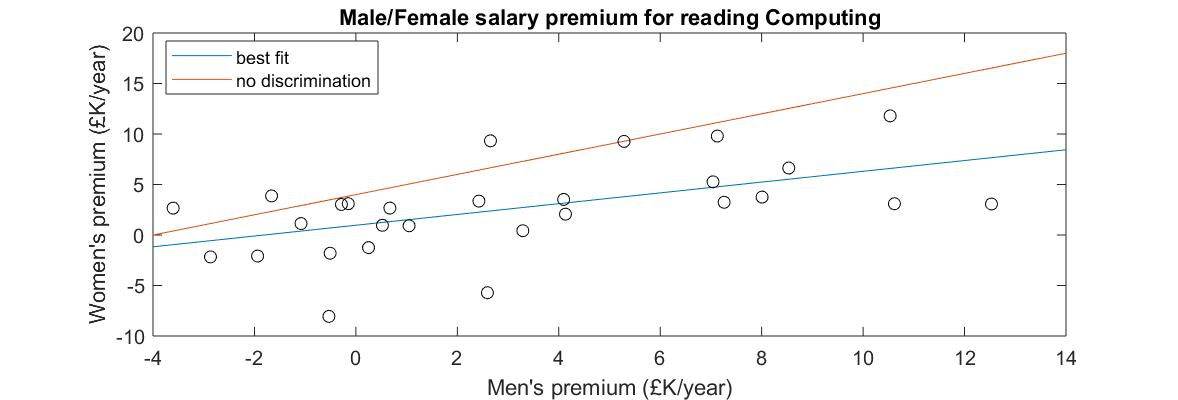
\includegraphics[scale=0.6]{images/BBCSalaryDatav6.jpg}}\noindent
Taking account of background and prior attainment, what a student would earn by reading computing at a specific university, versus reading a random subject at a random university. Data from \cite{DfE2018d}, matching tax and education records.
  }
%%%%%%%%%%%%%%%%%%%%%%%%%%%%%%%%%%%%%%%%%%%%%%%%%%%%%%%%%%%%%%%%%%%%%%%%%%%%%%
  \headerbox{Problem}{name=problem,column=0,below=earnings}{
%%%%%%%%%%%%%%%%%%%%%%%%%%%%%%%%%%%%%%%%%%%%%%%%%%%%%%%%%%%%%%%%%%%%%%%%%%%%%%
\noindent
 Superficially, the employment outlook for computing graduates in the
UK looks excellent. A 2015 report %from the UK Commission for Employment and Skills~
\cite[p.~74]{UKCES2015b} states:

\begin{quote} ...``{\emph{the digital sub-sector will need 518,000 workers for
roles in the three highest skilled occupational groups. However, over
the last ten years only 164,000 individuals graduated from a first
degree in computer science.}}''
\end{quote}

This is beneficial to the individual: according to %a 2011 UK Government report on economic returns from higher education qualifications~
\cite[Figure 4]{BIS2011a}, ``mathematical and
computer sciences'' have the second highest earnings return of all
subjects (overtaken only by ``medicine and dentistry'').  The country
profits from this as well: per head, it is the fourth most beneficial
subject to the UK~\cite[p.~16]{BIS2011a}. Nevertheless, the employment
figures are not great, and the earnings data are patchy \cite{Shadbolt2016a}. }

%%%%%%%%%%%%%%%%%%%%%%%%%%%%%%%%%%%%%%%%%%%%%%%%%%%%%%%%%%%%%%%%%%%%%%%%%%%%%%

%%%%%%%%%%%%%%%%%%%%%%%%%%%%%%%%%%%%%%%%%%%%%%%%%%%%%%%%%%%%%%%%%%%%%%%%%%%%%%

%%%%%%%%%%%%%%%%%%%%%%%%%%%%%%%%%%%%%%%%%%%%%%%%%%%%%%%%%%%%%%%%%%%%%%%%%%%%%%
  \headerbox{Institute of Coding}{name=IoC,column=0,below=problem}{
%%%%%%%%%%%%%%%%%%%%%%%%%%%%%%%%%%%%%%%%%%%%%%%%%%%%%%%%%%%%%%%%%%%%%%%%%%%%%%
{\setlength{\itemsep}{0pt}\setlength{\parsep}{0pt}
\begin{itemize}\setlength{\itemsep}{-3pt}
\item Concept announced %by George Osborne 
Nov 2015
\item Contest launched HEFCE March 2017 (somehow morphed to ``England'')
\item Announced by Prime Minister, Davos Jan 2018
\end{itemize}
%Consortium of universities, industry, outreach and professional bodies working together to address part of the digital skills gap

Key challenges that the IoC will address:
\begin{itemize}\setlength{\itemsep}{-3pt}
\item High UK demand for digital specialists (Additional 500K+ by 2022, \cite{Shadbolt2016a})
\item High 6-month unemployment for CS graduates from English Universities ($\sim$11\%, HESA, 2016)
\item 
Mixed Diversity and Inclusion 
\item[+]50\% more from Low Participation Neighbourhoods than other STEM
\item[$-$]percentage of women graduating in CS in 2016/17 only 15\%
\end{itemize}
  }}

  \headerbox{References}{name=references,column=3,above=bottom}{
%%%%%%%%%%%%%%%%%%%%%%%%%%%%%%%%%%%%%%%%%%%%%%%%%%%%%%%%%%%%%%%%%%%%%%%%%%%%%%
    \smaller
    \bibliographystyle{plain}
    \renewcommand{\section}[2]{\vskip 0.05em}
     \bibliography{../ITiCSE2019}
   \vspace{0.3em}
  }


%%%%%%%%%%%%%%%%%%%%%%%%%%%%%%%%%%%%%%%%%%%%%%%%%%%%%%%%%%%%%%%%%%%%%%%%%%%%%%
\headerbox{Theme 1}{name=theme1,column=1,span=2,below=earnings}{\vskip-25pt
\vbox{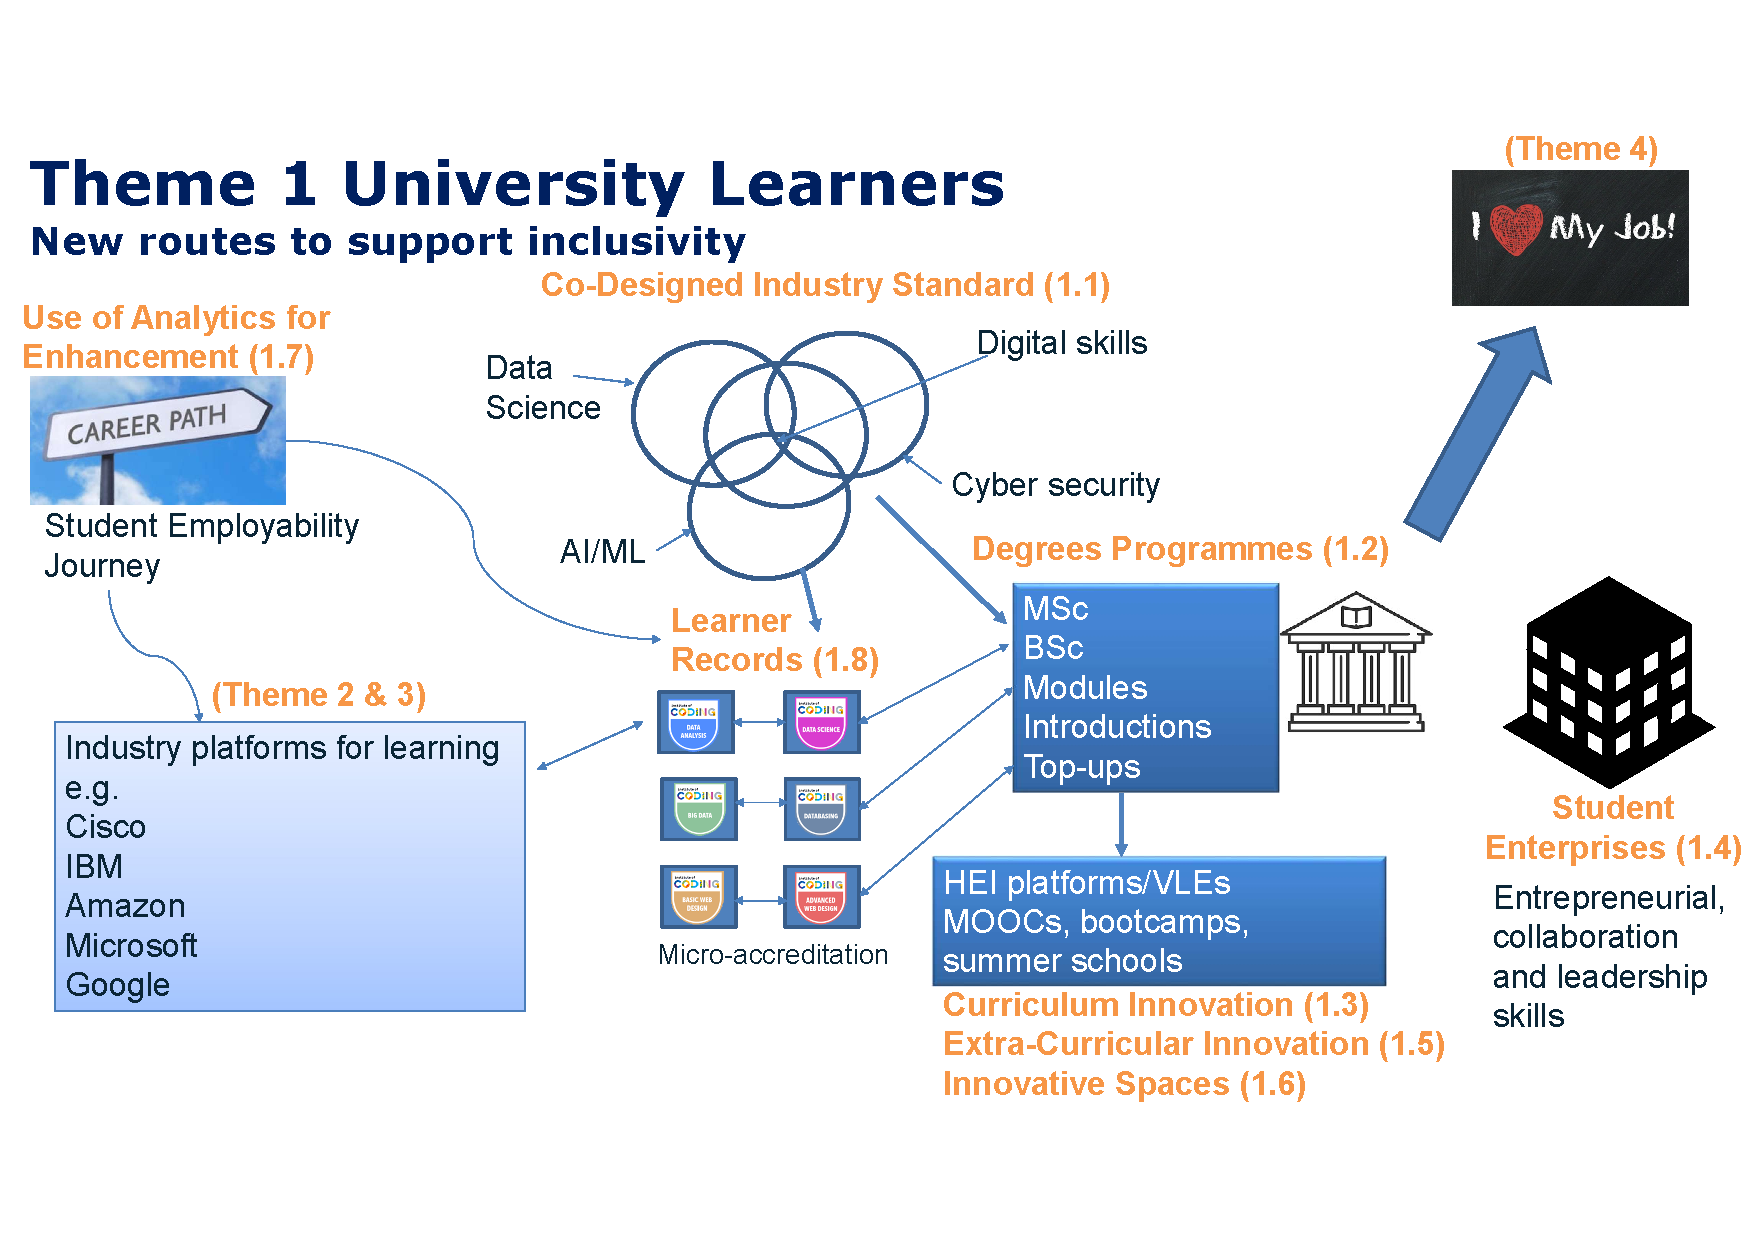
\includegraphics[scale=0.45]{images/Theme1.pdf}\vskip-40pt}
}

\headerbox{Structure}{name=solution,column=1,row=0,below=theme1}{
  %%%%%%%%%%%%%%%%%%%%%%%%%%%%%%%%%%%%%%%%%%%%%%%%%%%%%%%%%%%%%%%%%%%%%%%%%%%%%%
\noindent
 Consortium of universities, industry, outreach and professional bodies working together %to address part of the digital skills gap, targeting four key groups
 through the 5 themes:
\begin{enumerate}\setlength{\itemsep}{-3pt}
\item {\bf University Learners}: %led by the Open University 
Increase the number of university learners and improve employability %through innovative learning methods
\item {\bf The Digital Workforce}: %led by Aston University 
 create work-based learning that meets employer and student needs %, enriches the student experience and provide in-work and flexible learning options %that are viable at scale
\item {\bf Digitalising Professions}: %led by Coventry University 
develop learning to address sector specific digital skills needs \& modular training; Short courses and CPD for industries other than IT: creative economy, automotive, manufacturing, healthcare, the financial sector etc.
\item {\bf Widening Participation}: %led by QMUL 
\item {\bf Sharing and Sustainability}: %led by the University of Bath 
horizon scan for future digital skills need, disseminate and share best practice.% of the project.
%, look at long-term sustainability and the management of the programme
\end{enumerate}

  }
\headerbox{Theme 2}{name=theme2 ,column=2,row=0,below=theme1}{
\begin{description}\setlength{\itemsep}{-3pt}
\item[Aim:]to create a new industry-facing market of HEI-led, industry-valued provision % in areas of strategic importance 
\item[2.1]Alternative Delivery Models:
		identify and synthesis good practice 

\item[2.2]Specialist Provision:
	to upskill employees with an existing technical background in the area
\item[2.3]Generalist Provision: 
	retrain employees from different background with digital skills to move into 	new roles
\item[2.4]Education training:
	to work with employers on training employees with an educational role in their company.
\end{description}%\vskip -10pt
}
\headerbox{Theme 4}{name=theme4 ,column=2,row=0,below=theme2}{
Develop a path from first contact (overlap with schools projects) to employment, understanding and removing barriers to entry and progress for poorly served groups

}
\end{poster}

\end{document}

